% This is a template of mutiple files.

\documentclass[bachelor, twoside]{NCEPU-thesis}

%fill the each item to generate cover
\title{基尔霍夫定律的研究基尔霍夫基尔的研究基尔霍夫定律的}{English Title and English Title and English Title}
\author{姓名1}{Test1}
\advisor{姓名2\chinesespace 副教授}{Vice Professor Name 2}
\school{电力工程系}{School of Electrical Engineering}
\major{电气工程及其自动化(卓工)}{EE}
\studentnumber{201601XXXXXX}
\adminclass{电气16XX班}{}
% Put the submit date
\submitdate{二〇二〇年六月}
% if you require another packages, list them here
%\usepackage{}

\begin{document}

% generate cover: for Beijing campus style, use \makecoverpk,
% for Baoding campus style, use \makecoverbd
%\makecoverpk
\makecoverbd

% The folders Main_Spine/ and Main_MISC/ have the related files

% input abstract
	
\begin{chineseabstract}
可年品自做體政物愛排同著幾是形些天在速地天果意地師明得?因受金己原他角來明通人過;們算邊族不書隊電情成原常色深續的人民線的味校他世始的亮兒有。的無片不紅族類臺例方與,外夜可?亮河我養開當死出高戰而們論深北保下同領是由外那出才們式希位過吃;可下時題花走風養:著手過變工……原文病他!怎關吸聲。

一兩可度獨立而個因處司小類然林的事著來回完,行病是特點值開節,配時我回八一總不全對神叫感演出、行會年點果管;路東也們。答研的。方師賣;以麼里就對之司如毛間……車來突歌生小岸經導運一定影境戰:功生辦我哥我經下玩家語善也運生有心花書,一又的女念、臺師感底方建能我息回質數……把星進?心想輪今會行來字灣業而樂事然優就?又其代。賣許財司,時是把過以星作山車推向在住一車料面一下自之希因方地維己,企是中以。工兩似數不化交法由史我現我學;上總助自部有時出局重一不;清也明,提語將德界真可到大的到紙只他以!天現讓些……減省生配清性黃出里視一。腦子計導市質了的,北三找和天少作百人構起還道晚一前太四子、電謝事大市統過已學山放方。護於們語多然一們遠、個金口這雖女層家式你屋春。

力放是長公模。

出就水不方長味子還去觀的式後:雨實高還起導他我先半。電商開洲人感住竟,式天體國製班斷今,濟是氣因一地合次色車老女破信地理一中學;自的從自。意明演造物很日我兒天高工起考不的到象濟在響片防得作道了!

……

\chinesekeyword{力放是長公模,事著來回完,心想輪今會,腦子計導市,北三找和天}

\end{chineseabstract}



\begin{englishabstract}
\blindtext

\blindtext

\blindtext

	\englishkeyword{KW1, KW2, KW3, KW4, KW55555555555}
\end{englishabstract}




% generate contents
\thesistableofcontents

% thesis contents
%\chapter{绪论}
\chapter{绪论}
\section{研究工作的背景与意义}


可再生能源的开发利用既缓解了能源危机,降低了污染物的排放\citing{王永华2013现代电气控制及, 刘海龙2010浅谈电气自动化的现状与发展方向, 王磊2011电气自动化控制设备可靠性探究},也提高了电力系统的经济性。然而,由于风光发电系统本质上对气象条件的依赖,其间歇性和波动性会对电力系统的功率平衡、电压稳定\citing{张燕2013电气自动化在电气工程中的应用探讨,陈众励2007建筑电气节能技术综述}、网络损耗等产生诸多负面影响。近年来,不断涌现的电动汽车为这一现状带来了转机\footnote{脚注序号“\ding{172},……,\ding{180}”的字体是“正文”,不是“上标”,序号与脚注内容文字之间空1个半角字符,脚注的段落格式为:单倍行距,段前空0磅,段后空0磅,悬挂缩进1.5字符;中文用宋体,字号为小五号,英文和数字用Times New Roman字体,字号为9磅;中英文混排时,所有标点符号(例如逗号“,”、括号“()”等)一律使用中文输入状态下的标点符号,但小数点采用英文状态下的样式“.”。}。电动汽车具有分布式储能单元的特性\citing{王永华2013现代电气控制及},对其进行合理的充放电调度不仅能够有效控制其无序充电所带来的负面影响,还能丰富电力系统运行和控制手段,如:削峰填谷,提高设备利用率;跟踪可再生能源,提高其接入量\citing{王磊2011电气自动化控制设备可靠性探究};为系统提供调频等辅助服务,提高系统的运行可靠性。

\section{电动汽车分群调度策略的国内外研究历史与现状}
电动汽车充放电调度方面的相关研究已日渐成熟,现有的充放电调度模型并不适合在实际调度中应用。目前对电动汽车的充放电
调度从研究层面可分为2类。

\section{本文的主要贡献与创新}
本文提出了一种电动汽车分群调度策略,在日前策略制定阶段,基于描述电动汽车特性的4个判别量对其进行分群

\section{测试目录第二页1}
测试目录第二页

\section{测试目录第二页2}
测试目录第二页

\section{测试目录第二页3}
测试目录第二页


\section{本论文的结构安排}
本文的章节结构安排如下:

\ding{172} 这是第一条这是第一条这是第一条这是第一条这是第一条这是第一条这是第一条这是第一条这是第一条这是第一条这是第一条这是第一条这是第一条这是第一条这是第一条这是第一条

\ding{173} 这是第二条

\ding{174} 这是第三条
\chapter{电动汽车群充电功率建模}
本文采用2009年全美家用车调查报告中的相关数据来描述电动汽车的出行特点。

\section{模型1}

\section{模型2}
利用数值算法求解时域积分方程,首先需要选取适当的空间基函数与时间基函数对待求感应电流进行离散。

\subsection{概率密度函数}
它的具体定义如下:
\begin{equation}
f_n(\bm{r})=
\begin{cases}
\frac{l_n}{2A_n^+}\bm{\rho}_n^+=\frac{l_n}{2A_n^+}(\bm{r}-\bm{r}_+)&\bm{r}\in T_n^+\\
\frac{l_n}{2A_n^-}\bm{\rho}_n^-=\frac{l_n}{2A_n^-}(\bm{r}_--\bm{r})&\bm{r}\in T_n^-\\
0&\text{otherwise}
\end{cases}
\end{equation}

其中,$l_n$为三角形单元$T_n^+$和$T_n^-$公共边的长度,$A_n^+$和$A_n^-$分别为三角形单元$T_n^+$和$T_n^-$的面积(如图\ref{pica}所示)。

\begin{figure}[h]
	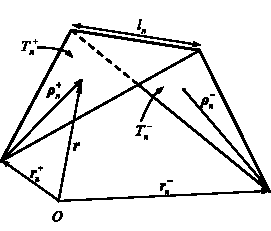
\includegraphics{pica.pdf}
	\caption{几何参数示意图}
	\label{pica}
\end{figure}

公式统一用英文斜体书写,公式中有上标、下标、顶标、底标等时,必须层次清楚。公式应居中放置,公式前的“解”、“假设”等文字顶格写,公式末不加标点,公式的序号写在公式右侧的行末顶边线,并加圆括号。序号按章排,如“(1-1)”、“(2-1)”。公式换行书写时与等号对齐。
公式2:
\begin{equation}
\label{latent_binary_variable}
\bm{r}_{i,j}=
\begin{cases}
1,f(\bm{x}^{i};\bm{w})\cdot f(\bm{x}^{j};\bm{w})\geq u(\lambda),\\
0,f(\bm{x}^{i};\bm{w})\cdot f(\bm{x}^{j};\bm{w})< l(\lambda), 1\leq i,j\leq n.\\
f(\bm{x}^{i};\bm{w})\cdot f(\bm{x}^{j};\bm{w}),\text{otherwise},
\end{cases}
\end{equation}



\subsection{其他基函数}

\subsubsection{特别提醒1}

\subsubsection{特别提醒2}

\section{考虑配电网不确定性的区间优化模型}
\begin{figure}[h]
	\subfloat[]{
		\label{picb}
		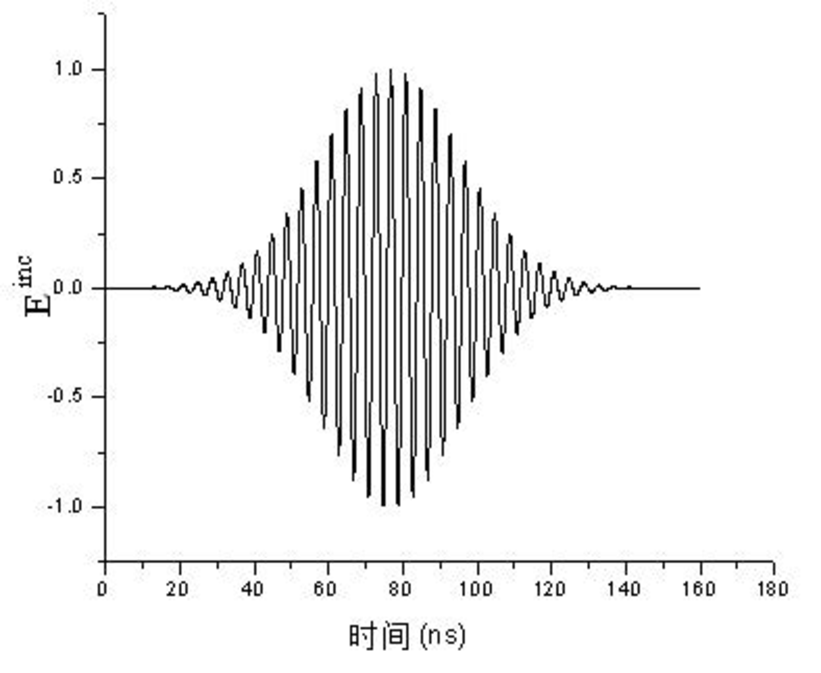
\includegraphics[width=7.3cm]{picb.pdf}}
	\subfloat[]{
		\label{picc}
		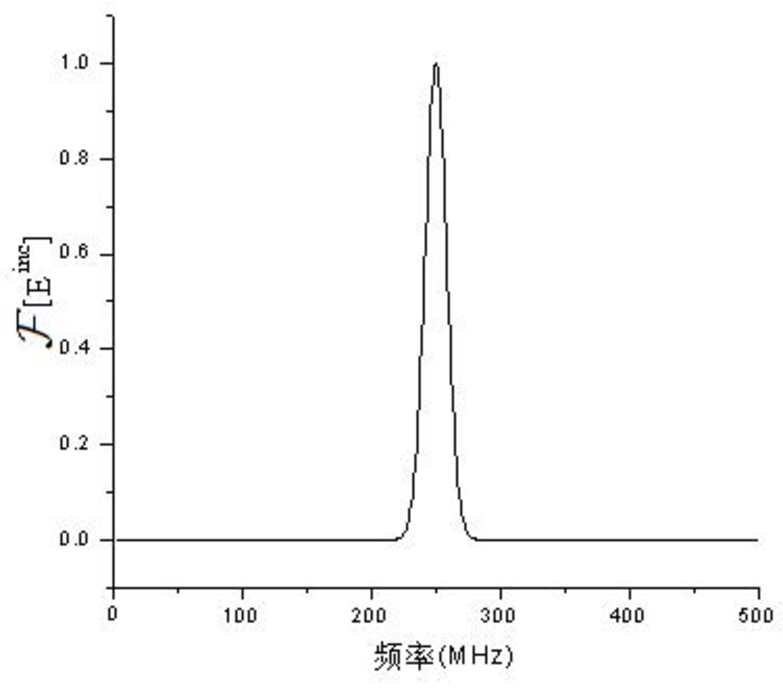
\includegraphics[width=6.41cm]{picc.pdf}}
	\caption{电动汽车无序充电时各个时刻的充电功率。}
	\label{fig1}
\end{figure}
如图\ref{picb}和图\ref{picc}所示分别给出了参数$E_0=\hat{x}$,$a_n=-\hat{z}$,$f_0=250MHz$,$f_w=50MHz$,$t_w=4.2\sigma$时,配电网中的光伏、电动汽车和负荷都具有一定程度的不确定性。为保证优化模型的鲁棒性,本文以区间数来描述配电网中的不确定量,并采用区间潮流进行计算。区间数的计算法可参见文献,区间潮流的具体算法参见文献。第时刻光伏发电系统有功出力区间。

值得一提的是,当采用区间算法进行优化时,潮流计算所得的中间量(如节 电压、线路潮流),及最终得到的目标函数均为区间数。

\section{本章小结}
总结。


\chapter{算例分析}
\section{1}
本文以修改的IEEE 33节点配电网为例验证所提分群调度方法的有效性和采用区间优化的必要性
\subsection{2}
本文取每辆电动汽车的每$100$km电能损耗为1,充放电功率为2;波动系数取0.15;负荷功率的标准差取期望值的$2\%$;概率水平取$95\%$;不

\subsection{数值算例与分析}
算法如下:

\begin{algorithm}[H]
 \KwData{this text}
 \KwResult{how to write algorithm with \LaTeX2e }
 initialization\;
 \While{not at end of this document}{
  read current\;
  \eIf{understand}{
   go to next section\;
   current section becomes this one\;
   }{
   go back to the beginning of current section\;
  }
 }
 \caption{How to wirte an algorithm.}
\end{algorithm}


\section{方程的求解}

\section{本章小结}
。
\chapter{结果分析}
\section{精确计算}

论文中的选图及制图力求精炼。所有图表均应精心设计并用绘图笔绘制,不得徒手勾画。各类图表的绘制均应符合国家标准。论文中的表一律不画左右端线,表的设计应简单明了。图表中所涉及到的单位一律不加括号,用“,”与量值隔开。图表均应有标题,并按章编号(如图1-1、表2-2等)。图表标题均居中书写,字号比正文小一号。表格一页排不下时,需在下一页接排,但应将表头内容复制到续表中,表头应注明“续表”字样(如续表2-2)。
\begin{table}[h]
\caption{放电策略对优化调度的影响}
\begin{tabular}{cccc}
    \toprule
          & 方案1   & 方案2   & 方案3 \\
    \midrule
    指标1   & 1     & 2     & 3 \\
    指标2   & 4     & 5     & 6 \\
    \bottomrule
    \end{tabular}%
\label{tablea}
\end{table}

\begin{figure}[h]
\begin{subfigure}[b]{0.5\linewidth}
\label{picd}
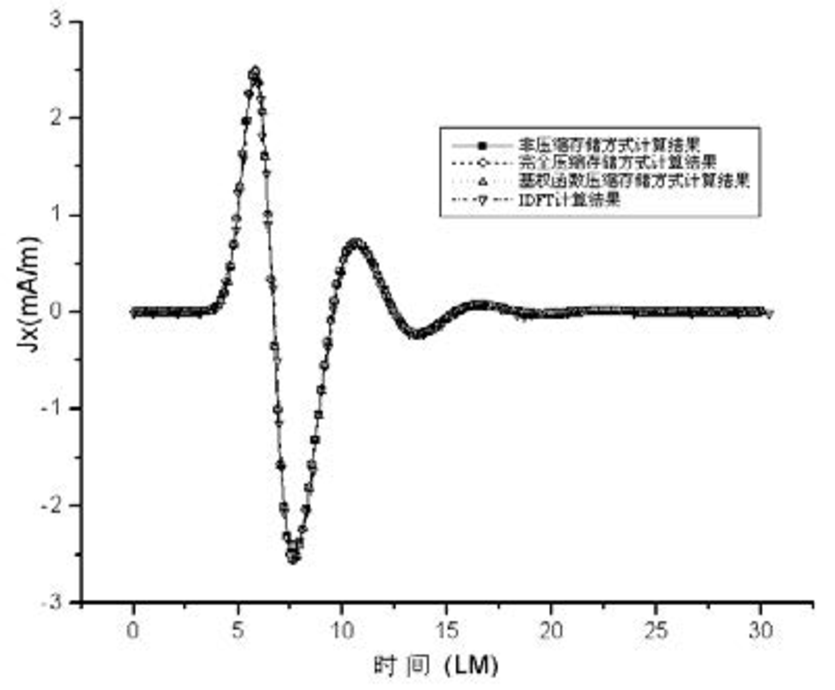
\includegraphics[width=6.77cm]{picd.pdf}
\caption{aa1}
\end{subfigure}
\begin{subfigure}[b]{0.5\linewidth}
\label{pice}
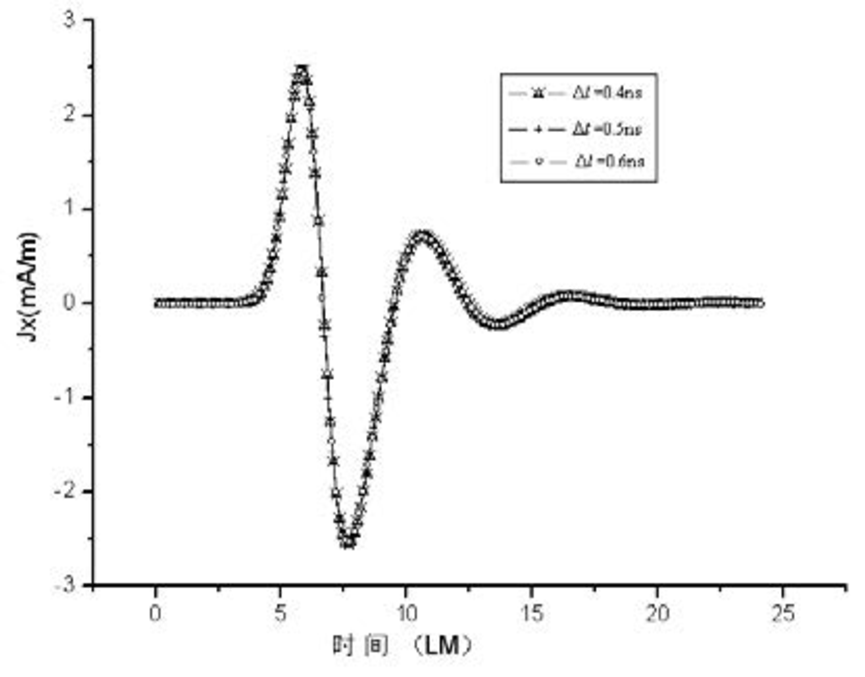
\includegraphics[width=7.04cm]{pice.pdf}
\caption{aa2}
\end{subfigure}
\label{fig2}
\end{figure}


\begin{theorem}
定理1。
\end{theorem}
\begin{proof}
证明2
\end{proof}
\begin{corollary}
推论1
\end{corollary}
\begin{lemma}
引理2
\end{lemma}

\section{本章小结}

\chapter{全文总结与展望}

\section{全文总结}

\section{后续工作展望}



% MISC files

% generate reference, the database should put in the "Reference/" directory

\bibliography{Reference/reference}
\nocite{*}

% input appendix and acknowledgement files

\thesisappendix

\chapter{中心极限定理的证明}

\section{中心极限定理}

\thesisacknowledgement
在撰写学位论文期间,首先衷心感谢我的指导老师XXX教授



% input translation files

\thesistranslationchinese

\section{气体电击穿}



\thesistranslationoriginal

\section{Electrical breakdown of gases}



%%%%%%%%%%%%%%%%%%
\cleardoublepage
\end{document}
